\documentclass[a4paper, 12pt]{article}%тип документа

%Русский язык
\usepackage[T2A]{fontenc} %кодировка
\usepackage[utf8]{inputenc} %кодировка исходного кода
\usepackage[english,russian]{babel} %локализация и переносы

%отступы 
\usepackage[left=2cm,right=2cm,top=2cm,bottom=3cm,bindingoffset=0cm]{geometry}

%Вставка картинок
\usepackage{graphicx}
\graphicspath{}
\DeclareGraphicsExtensions{.pdf,.png,.jpg, .jpeg}

%Таблицы
\usepackage[table,xcdraw]{xcolor}
\usepackage{booktabs}

%Графики
\usepackage{pgfplots}
\pgfplotsset{compat=1.9}
\usepackage{wrapfig}

%Математика
\usepackage{amsmath, amsfonts, amssymb, amsthm, mathtools}

%Заголовок
\author{Нугманов Булат}
\title{ 123 \\ Резонанс токов}

\begin{document}
\maketitle

\section*{Оборудование}
Генератор синусоидального напряжения, осциллограф, вольтметры, магазин ёмкостей.
\section*{Teория}
$I=\dfrac{E}{R_I}=\dfrac{E_0cos(\omega t+\varphi_0)}{R_I}=I_0cos(\omega t+\varphi_0)$ --- ток на генераторе.\newline
$$R_S=\dfrac{U_{RS}}{I}=\frac{U_{RS}}{\omega CU_{CS}}=\dfrac{1}{\omega C}tg\delta$$
где $R_S$ - эквивалентное последовательное сопротивление (ЭПС).\newline
Для используемых емкостей $C_n$ выполнено $tg\delta<10^{-3}$.\newline
$$R_{\sum}=R+R_L+R_S$$
где $R_{\sum}$ - суммарное активное сопротивление контура.\newline
Воспользуемся методом комплексных амплитуд:\newline
$Z_L=R_L+i\omega L$, $Z_C=R_S-i\frac{1}{\omega C}$, $Z=R_{\sum}+i(\omega L-d\dfrac{1}{\omega C})$.\newline
Тогда напряжение на контуре и токи на индуктивной и емкостной частях контура при нулевой начальной фазе можно предствить в виде:\newline
$$I_c=I\dfrac{Z_L}{Z_C+Z_L}=iQI_0\dfrac{\omega}{\omega_0}\dfrac{1-i\dfrac{R+R_L}{\rho}\dfrac{\omega_0}{\omega}}{1+iQ(\dfrac{\omega}{\omega_0}-\dfrac{\omega_0}{\omega})}$$
$$I_L=I\dfrac{Z_c}{Z_C+Z_L}=iQI_0\frac{\omega_0}{\omega}\frac{1+itg\delta}{1+iQ(\frac{\omega}{\omega_0}-\frac{\omega_0}{\omega})}$$
$$U=I\frac{Z_LZ_c}{Z_C+Z_L}=Q\rho I_0\frac{(1-i\frac{R+R_L}{\rho}\frac{\omega_0}{\omega})(1+itg\delta)}{1+iQ(\frac{\omega}{\omega_0}-\frac{\omega_0}{\omega})}$$
где $\omega_0=\frac{1}{\sqrt{LC}}$ - собственная частота, $\rho=\sqrt{\frac{L}{C}}$ - реактивное сопротивление контура, $Q=\frac{\rho} {R_{\sum}}$ --- добротность контура.\newline
Рассмотрим случай, когда $|\Delta\omega|=|\omega-\omega_0|\ll\omega_0$. Тогда
$$\frac{\omega}{\omega_0}-\frac{\omega_0}{\omega}=\frac{2\Delta\omega}{\omega_0}$$
Пренебрегая поправками порядка $Q^{-2}$, получим:
$$I_c=QI_0\frac{\omega}{\omega_0}\frac{e^{i\phi_c}}{\sqrt{1+(\tau\Delta\omega)^2}},    \phi_c=\frac{\pi}{2}-\frac{R+R_L}{\rho}-arctg(\tau\Delta\omega)$$
$$I_L=QI_0\frac{\omega_0}{\omega}\frac{e^{i\phi_L}}{\sqrt{1+(\tau\Delta\omega)^2}}, \phi_L=-\frac{\pi}{2}+\delta\arctg(\tau\Delta\omega)$$
$$U=Q\rho I_0\frac{\omega}{\omega_0}\frac{e^{i\phi_U}}{\sqrt{1+(\tau\Delta\omega)^2}}, \phi_U=-\frac{\omega}{\omega_0}\frac{R+R_L}{\rho}+\delta-arctg(\tau\Delta\omega)$$
где $\tau=\frac{2L}{R_{\sum}}=\frac{2Q}{\omega_0}$ - время затухания.\newline
При резонансе, т.е. когда $\Delta\omega=0$:
$$I_c(\omega_0)=QI_0, \phi_c(\omega_0)=\frac{\pi}{2}-\frac{R+R_L}{\rho}$$
$$I_L(\omega_0)=QI_0, \phi_L(\omega_0)=-\frac{\pi}{2}+\delta$$
$$U(\omega_0)=Q\rho I_0=Q^2R_{\sum}I_0, \phi_U{\omega_0}=-\frac{R+R_L}{\rho}+\delta$$
$$\phi'_c(\omega_0)=\phi'_L(\omega_0)=\phi'_U(\omega_0)=-\tau$$.

\section*{Эксперимент}

В работе исследуется следующая схема:
\begin{center}
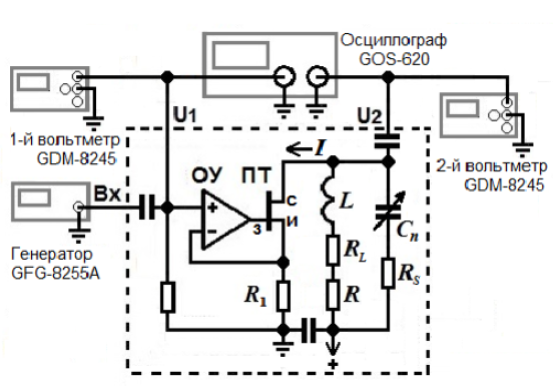
\includegraphics[width=0.6\textwidth]{U.png}\\
\textbf{Рис. 1} Установка.
\end{center}

$R=3.5$ Ом,
$R_1 = 1008$ Ом.
\section*{Параметры установки}
Установим такую амплитуду колебаний на генераторе, чтобы на 1 вольтметре было среднеквадратическое значение $E$. Проведём эксперимент при $E=0.2$ В и $E=0.1$ В для 7 различных ёмкостей. Также определим суммарное сопротивление, активное сопротивление катушки, ёмкость катушки, максимальное сопротивление конденсатора. Результаты представлены в таблице. 
\begin{table}[!ht]
\center
\begin{tabular}{|c|c|c|c|c|c|c|}
\hline
\multicolumn{7}{|c|}{$C,$ мкФ}                  \\ \hline
25.1 & 33.2 & 47.3 & 57.4 & 67.5 & 82.7 & 101.6 \\ \hline
\end{tabular}
\end{table}


\[L=\frac{1}{C(2\pi f)^2} \]
\[\rho=\frac{1}{2\pi fC} \]
\[Z_{\text{рез}}=\frac{U}{E_0}R_1\]
\[Q=\frac{UR_1}{E_0}2\pi fC\]
\[R_{\sum}=\frac{E_0}{UR_1}\frac{1}{(2\pi fC)^2}\]
\[R_{Smax}=10^{-3}\cdot\frac{1}{\omega_0C}\]
\[R_L=\frac{E_0}{UR_1}\frac{1}{(2\pi fC)^2}-R-10^{-3}\cdot\frac{1}{\omega_0C}\]

\begin{table}[!ht]
\center
\caption{$E=0.2$ В}
\begin{tabular}{|c|c|c|c|c|c|c|c|c|c|}
\hline
\rowcolor[HTML]{C0C0C0}
 & $E, \text{В}\cdot 10^{-3} $ & $U, \text{В}\cdot 10^{-3} $ & $f, \text{кГц}$ & $L, \text{мкГн}$ & $\rho, \text{Ом}$ & $Z_{res}, \text{Ом}\cdot 10^{3} $ & $Q$ & $R_L, \text{Ом}$ & $R_{\sum}, \text{Ом}$ \\ \hline
\cellcolor[HTML]{C0C0C0} 1 & 200 & 1000 & 32 & 970 & 200 & 5.2 & 26 & 3.7 & 7.4 \\ \hline
\rowcolor[HTML]{EFEFEF} 
\cellcolor[HTML]{C0C0C0} 2 & 200 & 810 & 28 & 970 & 170 & 4.1 & 24 & 3.5 & 7.2 \\ \hline
\cellcolor[HTML]{C0C0C0} 3 & 200 & 590 & 24 & 970 & 140 & 3 & 21 & 3.2 & 6.9 \\ \hline
\rowcolor[HTML]{EFEFEF} 
\cellcolor[HTML]{C0C0C0} 4 & 200 & 490 & 21 & 960 & 130 & 2.5 & 19 & 3.1 & 6.7 \\ \hline
\cellcolor[HTML]{C0C0C0} 5 & 200 & 420 & 20 & 970 & 120 & 2.1 & 18 & 3.1 & 6.7 \\ \hline
\rowcolor[HTML]{EFEFEF} 
\cellcolor[HTML]{C0C0C0} 6 & 200 & 350 & 18 & 970 & 110 & 1.8 & 16 & 3 & 6.6 \\ \hline
\cellcolor[HTML]{C0C0C0} 7 & 200 & 290 & 16 & 970 & 97 & 1.5 & 15 & 2.9 & 6.5 \\ \hline
\end{tabular}
\end{table}



\begin{table}[!ht]
\center
\caption{$E=0.1$ В}
\begin{tabular}{|c|c|c|c|c|c|c|c|c|c|}
\hline
\rowcolor[HTML]{C0C0C0}
 & $E, \text{В}\cdot 10^{-3} $ & $U, \text{В}\cdot 10^{-3} $ & $f, \text{кГц}$ & $L, \text{мкГн}$ & $\rho, \text{Ом}$ & $Z_{res}, \text{Ом}\cdot 10^{3} $ & $Q$ & $R_L, \text{Ом}$ & $R_{\sum}, \text{Ом}$ \\ \hline
\cellcolor[HTML]{C0C0C0} 1 & 100 & 520 & 32 & 970 & 200 & 5.2 & 27 & 3.6 & 7.4 \\ \hline
\rowcolor[HTML]{EFEFEF} 
\cellcolor[HTML]{C0C0C0} 2 & 100 & 410 & 28 & 970 & 170 & 4.1 & 24 & 3.4 & 7.1 \\ \hline
\cellcolor[HTML]{C0C0C0} 3 & 100 & 300 & 24 & 960 & 140 & 3 & 21 & 3.2 & 6.8 \\ \hline
\rowcolor[HTML]{EFEFEF} 
\cellcolor[HTML]{C0C0C0} 4 & 100 & 250 & 21 & 960 & 130 & 2.5 & 19 & 3.1 & 6.7 \\ \hline
\cellcolor[HTML]{C0C0C0} 5 & 100 & 210 & 20 & 960 & 120 & 2.1 & 18 & 3.1 & 6.7 \\ \hline
\rowcolor[HTML]{EFEFEF} 
\cellcolor[HTML]{C0C0C0} 6 & 100 & 180 & 18 & 960 & 110 & 1.8 & 16 & 3 & 6.6 \\ \hline
\cellcolor[HTML]{C0C0C0} 7 & 100 & 140 & 16 & 970 & 97 & 1.5 & 15 & 3 & 6.5 \\ \hline
\end{tabular}
\end{table}

Усреднив полученные значения, получаем, что $L=966 \pm 6$ мГн, $R_L=3.20 \pm 0.05$ Ом.
\subsection*{Резонансная кривая}
Теперь снимем резонансную кривую % что это и почему
Для определения точки резонанса проведём параболу по трём верхним точкам. Точку максимума параболы будем считать максимумом нашей кривой. 

\begin{center}
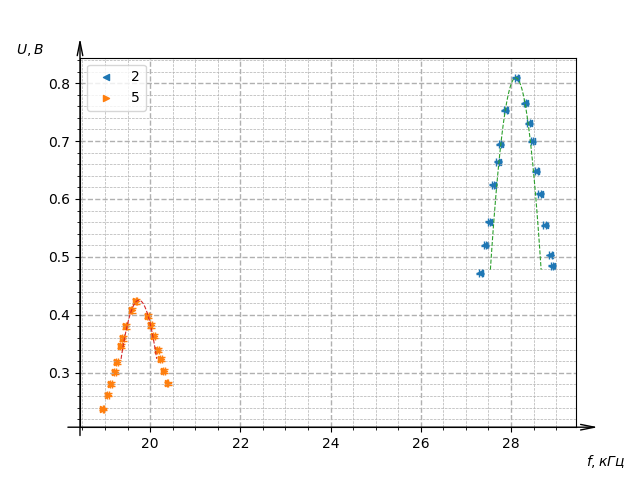
\includegraphics[width=\textwidth]{Figure_1.png}\\
\textbf{Рис. 2} Резонансные кривые для 2 режимов.
\end{center}

\begin{center}
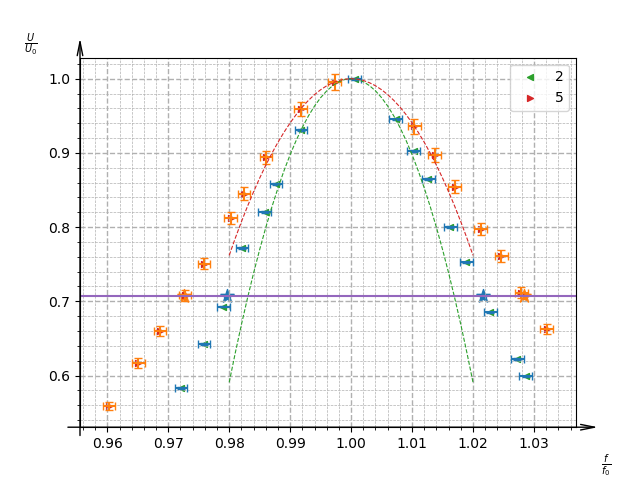
\includegraphics[width=\textwidth]{Figure_2.png}\\
\textbf{Рис. 3} Отнормированные резонансные кривые.
\end{center}

Как известно, добротность можно найти графически. На уровне $\frac{1}{\sqrt{2}}$ проведём прямую и определим "ширину" кривой. Для нахождения точки пересечения кривой с "уровнем" применим аппроксимацию прямой по двум близлежащим точкам. Таким образом, по ширине $\delta$, добротность находится так:

\[Q=\frac{1}{\delta}\]


Для наших кривых:
$Q_2 \approx 23.6$, 
$Q_5 \approx 19.1$.
\subsection*{Сдвиг фаз}
Перейдём к следующей части эксперимента. % Фазовый сдвиг и всё такое....

В точке резонанса сдвиг фаз определим, как $\pi$. По сути это безразлично, так как все фазы определяются с точностью до $\pi$.

\begin{center}
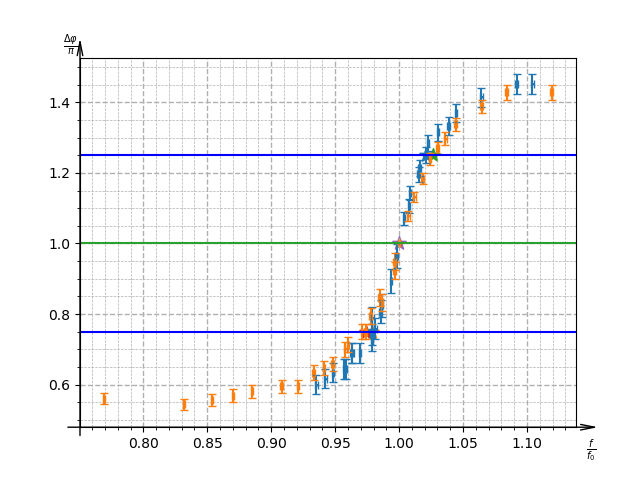
\includegraphics[width=\textwidth]{Figure_3.png}\\
\textbf{Рис. 4} Сдвиг фаз в зависимости от отноромированной частоты.
\end{center}

Также определим добротность графически. Для этого посчитаем точки пересечения с линиями уровней $\frac{3\pi}{4}$ и $\frac{5\pi}{4}$.

Для нахождения точки пересечения "уровня" с кривой всё также применяем аппроксимацию прямой по близлежащим точкам. Считая $Q$ по той же формуле, находим 
$Q_2 \approx 23.8$, 
$Q_5 \approx 18.0$.

\section*{$R_L(f)$}
Напоследок заметим, что $R_L(f)$, рассчитанное нами в первой части, не является в самом деле константой. Из-за скин-эффекта при повышении частоты, повышается также и эффективное сопротивление катушки.
\begin{center}
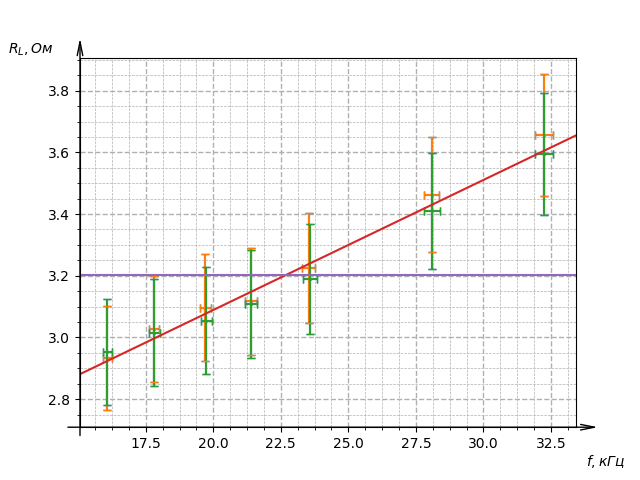
\includegraphics[width=\textwidth]{Figure_4.png}\\
\textbf{Рис. 5} Рост $R_L$ из-за скин-эффекта.
\end{center}

Если это как-то полезно, то при аппроксимации зависимости прямой, в 0 она достигает $2.246 \pm 0.038$ Ом.

\subsection{Векторная диаграмма}

Теперь построим векторную диаграмму. 

\begin{wrapfigure}{l}{0.34\linewidth} 
	\begin{tikzpicture} [scale = 1.8, yshift=2pt]
		\draw  (0, 0) -- (0, 2.1);
		\draw (0, 0) -- (0, - 2.1);
		\draw  (0, 0) -- (2.5, 0);
		\draw [->] (0, 0) -- (0.75, 2) node[anchor=west] {$ \vec{I_C} $};
		\draw (0, 1.3) arc (60:0: 0.6);
			\draw (0.2,1.4) node {$ \phi_C'$};
				\draw [->] (0, 0) -- (0.06, -2) node[anchor=west] {$ \vec{I_L} $};
			\draw (0, -1.3) arc (0:30: -0.4);
			\draw (0.15,-1.4) node {$ \delta$};
			\draw [->] (0, 0) -- (0.75, 0) node[anchor=south] {$ \vec{I} $};
			\draw [->] (0, 0) -- (1.75, -0.4) node[anchor=north] {$ \vec{U} $};
				\draw (1, 0) arc (30:0: 0.6);
					\draw (1.3,-0.2) node {$ \phi_U$};
	\end{tikzpicture}
\end{wrapfigure}

Посчитаем ток $ I = \dfrac{E}{R_1} = \dfrac{0,2 \text{В}}{1008 \text{Ом}} \approx 0,1 $ мА. Его вектор равен сумме: $ \vec{I} = \vec{I_L} + \vec{I_C} $, причем сам $ \vec{I} $ расположен на оси абсцисс, а его компоненты расположены к нему под углами

\[\phi_C = \dfrac{\pi}{2} - \dfrac{R + R_l}{\rho}, \quad \phi_L = -\dfrac{\pi}{2} + \delta\]

Здесь $ \delta \simeq 10^{-3}$ --- очень малый параметр установки, которым допустимо пренебречь при расчёте, однако можно изобразить для наглядности. Подсчитаем угол $ \phi_C' =   \dfrac{R + R_L}{\rho} \approx 0,03 $. 

Аналогичный угол у напряжения $ \vec{U}: \phi_U = - \dfrac{R + R_L}{\rho} $. Т.е. оно незначительно отклоняется от оси абсцисс на отрицательный угол.

Изобразим это на рисунке.

\textbf{    } 

\textbf{    } 

\section*{Вывод}
Две методики определения добротности дали весьма схожие результаты, что не может не радовать. Мы также убедились, что $R_L$ действительно зависит от частоты. В общем, что просили показать, то показали. А чего не просили --- только мельком.
\end{document}
